\chapter{Analyse du Système Actuel et Exploration d'Alternatives Similaires}


\section{Introduction}

Dans les établissements universitaires, les laboratoires de recherche jouent un rôle fondamental dans le développement scientifique. Ces structures ont régulièrement besoin de ressources matérielles spécifiques pour mener à bien leurs projets. Or, la gestion actuelle des demandes d'achat est souvent manuelle, peu centralisée et difficile à suivre.

Dans ce contexte, la transformation numérique s’impose comme une solution pertinente. Ce projet de fin d’études vise à concevoir une plateforme web de gestion des demandes administratives et d’achat de matériel, apportant plus de transparence, de traçabilité et d’efficacité.

\section{Cadre du projet}

Ce travail est réalisé dans le cadre du Projet de Fin d’Études pour l’obtention de la licence en Informatique, spécialité Génie Logiciel, à la \textbf{Faculté des Sciences de Gabès (FSG)}. Il est mené en collaboration avec le laboratoire \textbf{IReSCoMath}, une unité de recherche multidisciplinaire relevant de cette faculté.

L’objectif principal est de développer une application web centralisant et automatisant le processus de demande, tout en assurant un suivi structuré et une validation hiérarchique par le directeur du laboratoire.

\section{Analyse de l’existant}

\subsection{Présentation du Laboratoire IReSCoMath}

Le laboratoire IReSCoMath (Ingénierie de la Recherche en Sciences, Communication et Mathématiques) regroupe des enseignants-chercheurs, doctorants et étudiants de master. Il intervient dans divers domaines tels que les mathématiques appliquées, l’informatique, les technologies de l’information et les sciences de gestion.

Il soutient activement les projets nécessitant du matériel ou un accompagnement administratif, ce qui justifie la nécessité de structurer les processus de demande.

\subsection{Les activités principales du laboratoire IReSCoMath}

Parmi les principales activités du laboratoire, on trouve :
\begin{itemize}
  \item La supervision de projets de fin d’études (PFE) et de thèses ;
  \item L’organisation de conférences et séminaires scientifiques ;
  \item La publication de travaux de recherche ;
  \item La gestion de projets financés.
\end{itemize}

\subsection{Critique de l’existant}

Le processus actuel repose sur des échanges informels (papier, e-mails), ce qui engendre plusieurs limites :
\begin{itemize}
  \item Manque de traçabilité des demandes ;
  \item Difficulté à suivre leur état d’avancement ;
  \item Retards dus aux validations manuelles ;
  \item Communication peu efficace entre les acteurs.
\end{itemize}

\subsection{La solution proposée}

Le projet propose une plateforme web avec les fonctionnalités suivantes :
\begin{itemize}
  \item Formulaires de demande adaptés selon le profil (étudiant master, doctorant, enseignant-chercheur, directeur) ;
  \item Validation unique par le directeur du laboratoire ;
  \item Notifications automatiques à chaque étape ;
  \item Suivi en temps réel de l’état des demandes ;
  \item Archivage structuré des demandes validées.
\end{itemize}


\section{Exploration des alternatives similaires}

\subsection{Systèmes de gestion universitaire intégrés}

Dans le cadre de notre étude comparative, nous avons analysé plusieurs solutions existantes répondant aux besoins de gestion administrative et académique dans les établissements d'enseignement supérieur.

\begin{enumerate}[label=\alph*)]

\item \textbf{Banner (Ellucian)}

\textbf{Description générale.} \\
Banner est une solution logicielle intégrée de gestion universitaire, adoptée par plus de 2,700 établissements à travers le monde. Elle propose une plateforme unifiée couvrant l'ensemble des besoins administratifs et académiques d'une institution d'enseignement supérieur.

\textbf{Couverture fonctionnelle.}
\begin{itemize}
\item Gestion financière ;
\item Gestion des ressources humaines ;
\item Gestion du parcours étudiant (inscription, notes, diplômes, etc.) ;
\item Gestion des subventions et projets de recherche.
\end{itemize}

\textbf{Points forts.}
\begin{itemize}
\item Solution éprouvée et riche fonctionnellement ;
\item Intégration poussée entre les modules ;
\item Support technique étendu ;
\item Interface configurable.
\end{itemize}

\textbf{Limites.}
\begin{itemize}
\item Complexité et lourdeur du système ;
\item Coûts de mise en œuvre et de maintenance élevés ;
\item Personnalisation limitée sans développements spécifiques ;
\item Interface utilisateur perçue comme obsolète.
\end{itemize}

\textbf{Système de notifications.}
\begin{itemize}
\item Notifications par courriel ;
\item Tableaux de bord personnalisables ;
\item Rapports automatisés.
\end{itemize}

\textbf{Écart fonctionnel avec les besoins ciblés.} \\
Malgré sa richesse fonctionnelle, Banner ne cible pas les processus spécifiques de gestion de demandes internes (matériel, stages, missions). Son périmètre trop large et sa complexité technique en font une solution inadaptée à une approche modulaire, souple et légère comme celle que nous visons avec notre solution.

\item \textbf{PeopleSoft Campus Solutions (Oracle)}

\textbf{Description générale.} \\
Solution internationale proposée par Oracle, PeopleSoft Campus Solutions offre une plateforme complète pour la gestion des services aux étudiants dans les grandes institutions.

\textbf{Couverture fonctionnelle.}
\begin{itemize}
\item Gestion des admissions, cours et examens ;
\item Facturation et finance étudiante ;
\item Ressources humaines et infrastructures ;
\item Gestion documentaire et analytique.
\end{itemize}

\textbf{Points forts.}
\begin{itemize}
\item Solution modulaire hautement configurable ;
\item Forte présence internationale ;
\item Intégration avec d'autres produits Oracle.
\end{itemize}

\textbf{Limites.}
\begin{itemize}
\item Coûts de licence et de maintenance très élevés ;
\item Complexité de déploiement ;
\item Requiert des compétences techniques avancées.
\end{itemize}

\textbf{Système de notifications.}
\begin{itemize}
\item Moteur de workflow et alertes configurables ;
\item Intégration avec emails et portails étudiants.
\end{itemize}

\textbf{Écart fonctionnel avec les besoins ciblés.} \\
Bien que très complet, PeopleSoft est disproportionné par rapport à notre besoin ciblé. Il serait surdimensionné pour un simple module de gestion de demandes internes tel que celui que propose notre solution.

\end{enumerate}

\subsection{Solutions spécifiques au secteur académique}
\begin{enumerate}[label=\alph*)]
\setcounter{enumi}{2}  % Commence à la lettre c

\item \textbf{GLPI avec plugin ESM (Education Service Management)}

\textbf{Description générale.} \\
GLPI est une solution open source de gestion des services informatiques, largement utilisée dans les établissements éducatifs. Grâce au plugin ESM, elle peut être adaptée aux besoins spécifiques de la gestion administrative et matérielle.

\textbf{Couverture fonctionnelle.}
\begin{itemize}
\item Gestion des tickets et des demandes ;
\item Inventaire du matériel ;
\item Gestion des contrats et documents ;
\item Rapports et statistiques.
\end{itemize}

\textbf{Points forts.}
\begin{itemize}
\item Solution gratuite et libre ;
\item Grande flexibilité et adaptabilité via des plugins ;
\item Interface simple et fonctionnelle ;
\item Bonne gestion documentaire intégrée.
\end{itemize}

\textbf{Limites.}
\begin{itemize}
\item Orientation initiale centrée sur l'informatique (ITSM) ;
\item Interface parfois austère et peu intuitive ;
\item Adaptation aux processus académiques nécessitant des développements sur mesure.
\end{itemize}

\textbf{Système de notifications.}
\begin{itemize}
\item Notifications automatiques par email ;
\item Alertes sur les délais de traitement ;
\item Rappels automatisés pour les intervenants.
\end{itemize}

\textbf{Écart fonctionnel avec les besoins ciblés.} \\
GLPI pourrait constituer une base technique intéressante, notamment pour la gestion des demandes de matériel. Cependant, il nécessiterait une personnalisation importante pour intégrer d'autres processus tels que les conférences, les missions ou les stages que couvre notre solution.

\item \textbf{SIGB (Système Intégré de Gestion de Bibliothèque) adapté}

\textbf{Description générale.} \\
Les SIGB sont des systèmes conçus pour la gestion des bibliothèques universitaires, mais certains peuvent être adaptés à des usages administratifs élargis, notamment en matière de suivi des acquisitions et de validation des demandes.

\textbf{Couverture fonctionnelle.}
\begin{itemize}
\item Gestion des acquisitions de ressources ;
\item Suivi des demandes internes ;
\item Gestion documentaire structurée ;
\item Processus de validation hiérarchisés.
\end{itemize}

\textbf{Points forts.}
\begin{itemize}
\item Gestion d'acquisition bien rodée ;
\item Processus de demande formalisé et clair ;
\item Interface familière pour les utilisateurs du secteur universitaire.
\end{itemize}

\textbf{Limites.}
\begin{itemize}
\item Portée fonctionnelle limitée au domaine bibliothécaire ;
\item Difficulté d'adaptation à d'autres types de demandes (missions, stages) ;
\item Technologies parfois obsolètes ou rigides.
\end{itemize}

\textbf{Système de notifications.}
\begin{itemize}
\item Notifications simples par courrier électronique ;
\item Personnalisation des alertes limitée.
\end{itemize}

\textbf{Écart fonctionnel avec les besoins ciblés.} \\
L'approche structurée des SIGB en matière d'acquisition est pertinente pour la modélisation des demandes de matériel. Toutefois, la solution reste insuffisante pour couvrir l'ensemble des processus ciblés par notre solution.


\end{enumerate}

\begin{table}[h]
\centering
\caption{Tableau comparatif des solutions}
\begin{tabular}{|p{3.5cm}|p{2.2cm}|p{2cm}|p{2.5cm}|p{2cm}|p{3cm}|}
\hline
\textbf{Solution} & \textbf{Configurable} & \textbf{Complexité} & \textbf{Difficulté de mise en place} & \textbf{Coûts} & \textbf{Limitations} \\
\hline
Banner (Ellucian) & Limité & Très élevée & Très difficile & Très élevés & Personnalisation restreinte \\
\hline
PeopleSoft Campus Solutions & Très configurable & Très élevée & Très difficile & Très élevés & Compétences techniques spécialisées requises \\
\hline
GLPI avec plugin ESM & Très configurable & Modérée & Modérée & Très faibles (gratuit) & Orientation ITSM, interface austère \\
\hline
SIGB adapté & Limité & Modérée & Difficile & Modérés & Portée fonctionnelle limitée, technologies obsolètes \\
\hline
\end{tabular}
\end{table}

% Légende 
\begin{itemize}
\item \textbf{Configurable :}
    \begin{itemize}
    \item Très configurable : Paramétrage étendu sans développement
    \item Configurable : Paramétrage standard possible
    \item Limité : Peu d'options de configuration
    \end{itemize}

\item \textbf{Complexité :}
    \begin{itemize}
    \item Très élevée : Nécessite expertise technique approfondie
    \item Élevée : Compétences techniques avancées requises
    \item Modérée : Formation technique nécessaire
    \end{itemize}

\item \textbf{Difficulté de mise en place :}
    \begin{itemize}
    \item Très difficile : Projet complexe, long délai
    \item Difficile : Nécessite accompagnement expert
    \item Modérée : Mise en œuvre avec ressources internes
    \end{itemize}

\item \textbf{Coûts :}
    \begin{itemize}
    \item Très élevés : Budget conséquent requis
    \item Élevés : Investissement important
    \item Modérés : Coût raisonnable
    \item Très faibles : Solution économique
    \end{itemize}
\end{itemize}

\section{Spécifications des besoins}

\subsection{Identification des acteurs}

Les principaux acteurs du système sont :
\begin{itemize}
  \item \textbf{Étudiant Master} ;
  \item \textbf{Doctorant} ;
  \item \textbf{Enseignant-Chercheur} ;
  \item \textbf{Directeur de laboratoire} (aussi validateur).
\end{itemize}

\subsection{Types de demandes}

Les utilisateurs peuvent soumettre différents types de demandes, notamment :
\begin{itemize}
  \item Achat de matériel ;
  \item Prêt de matériel ;
  \item Mission professionnelle ;
  \item Stage ;
  \item Participation à un événement scientifique ;
  \item Autres demandes administratives spécifiques.
\end{itemize}

\section{Méthode de gestion de projet}

\subsection{Approche Scrum}

Afin d'assurer une gestion flexible et adaptative du projet, nous avons opté pour la méthodologie Scrum. Cette approche agile permet de découper le développement en itérations courtes (2-3 semaines), avec des points d'étape quotidiens et des revues de sprint pour évaluer l'avancement.

\subsection{Outils utilisés}

Dans le cadre de la gestion des tâches, nous avons adopté \textbf{Trello} pour sa simplicité d'utilisation et ses fonctionnalités collaboratives. Cet outil nous a permis de structurer le travail en sprint (\textit{À faire}, \textit{En cours}, \textit{Terminé}) et de suivre en temps réel l'avancement de chaque activité.

\begin{figure}[H]
    \centering
    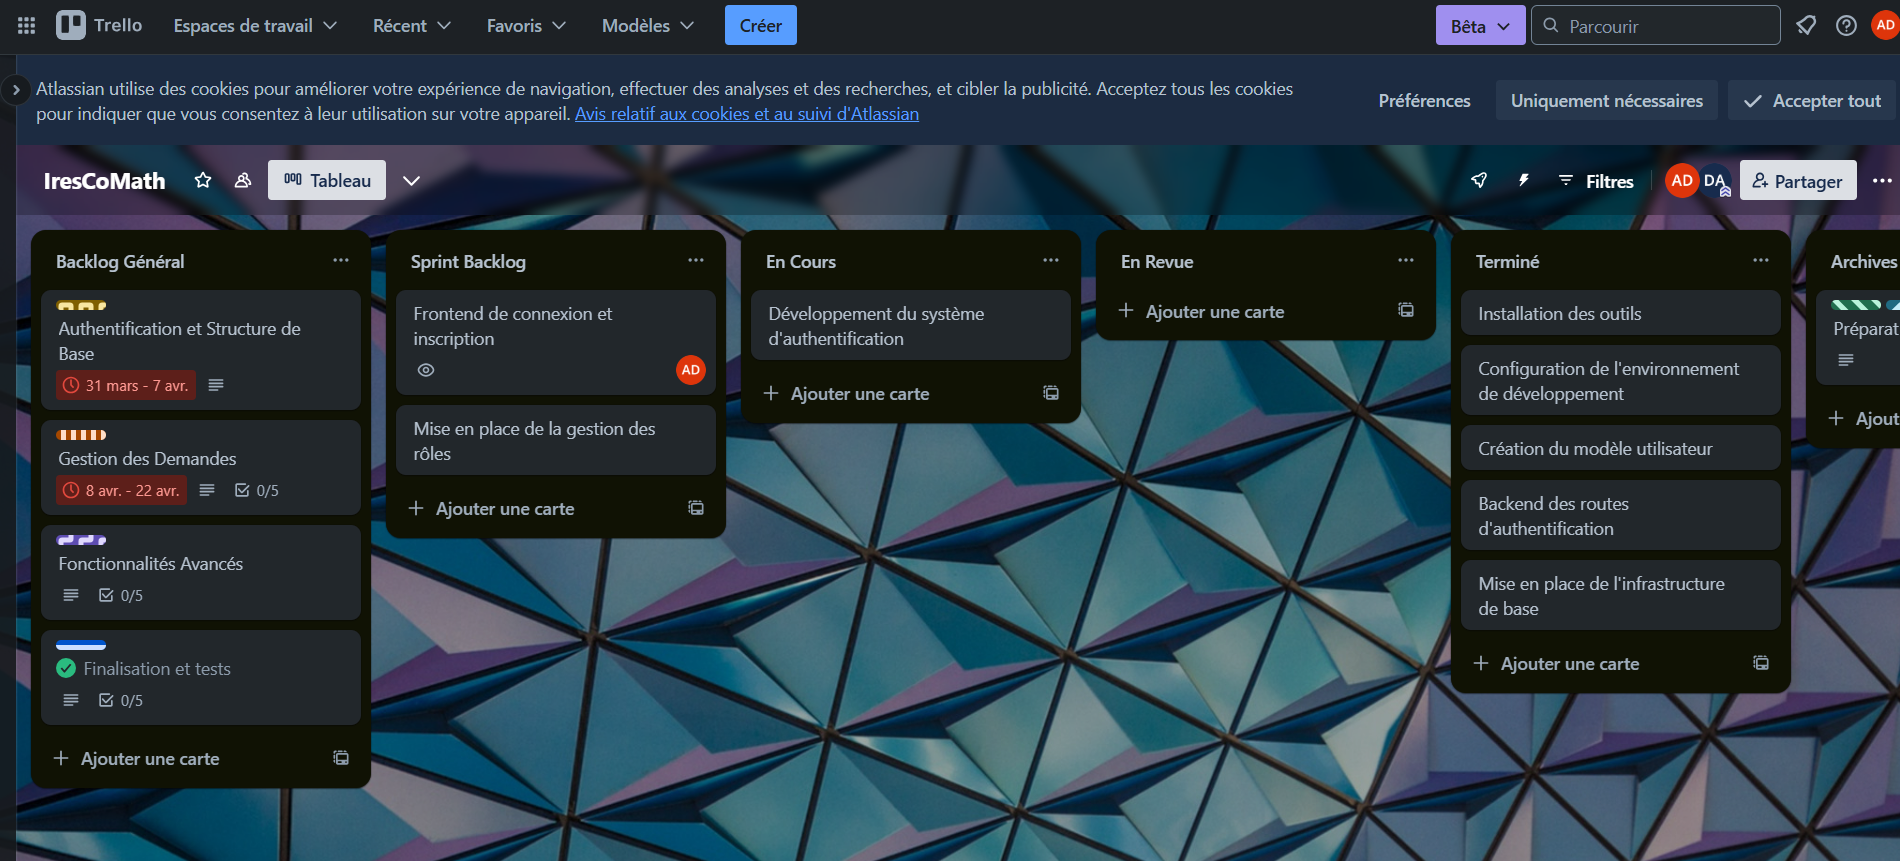
\includegraphics[width=0.8\textwidth]{images/Trello/Trello-Irescomath.png}
    \caption{Outils utilisés pour la gestion de projet}
    \label{fig:outils}
\end{figure}

Le projet a été structuré en sprints de 2 semaines :
\begin{itemize}
  \item \textbf{Sprint 1} : Architecture et authentification ;
  \item \textbf{Sprint 2} : Module de gestion des demandes ;
  \item \textbf{Sprint 3} : Workflow et notifications ;
  \item \textbf{Sprint 4} : Interface utilisateur et tests ;
  \item \textbf{Sprint 5} : Optimisations .
\end{itemize}
\section{Conclusion}

Ce premier chapitre a permis de poser les bases du projet en décrivant le contexte, les limitations du système actuel, les objectifs visés ainsi que la méthodologie utilisée. Le chapitre suivant portera sur la conception fonctionnelle et technique de la solution proposée.
